\documentclass[10pt,a4paper]{article}

\usepackage[scaled]{helvet}
\usepackage[left=2.5cm,right=2.5cm,top=3cm,bottom=3cm]{geometry}
\usepackage{parskip} % don't indent first line of paragraph
\usepackage[none]{hyphenat}\sloppy  % don't hyphenate
\usepackage{tocloft}\addtolength{\cftsubsubsecnumwidth}{0.5em}\tocloftpagestyle{fancy} % fix ToC spacing issue
\usepackage{float} % [H]
\usepackage{fancyref} % \Fref
\usepackage{csquotes} % \nquote
\usepackage{enumitem} % [nolistsep]
\usepackage[printonlyused,withpage]{acronym}
\usepackage{tabularx}
\usepackage{makecell}
\usepackage[table]{xcolor}
\usepackage[hidelinks]{hyperref}\hypersetup{colorlinks, allcolors=., urlcolor=teal}
\usepackage[skins]{tcolorbox}
\usepackage{fancyhdr}
\usepackage{titling} % \thetitle, \theauthor
\usepackage{longtable}
\usepackage{array} % \arraybackslash
\usepackage{multicol}
\usepackage{textcomp} % symbols, e.g. \textdegree
\usepackage{textgreek} % greek letters, e.g. \textmu
\usepackage[super]{nth}
\usepackage{sansmath}\sansmath
\usepackage{amsmath} % bmatrix
% \usepackage{svg}
\usepackage{macros} % project specific macros
\usepackage{subcaption}
\usepackage{tablefootnote}


\renewcommand\familydefault{\sfdefault}

\graphicspath{{images/}}  % Location of the graphics files

\pagestyle{fancy}
\fancyhf{}
\fancyhead[L]{\thetitle{} \version\\ \thedate}
\fancyfoot[R]{\thepage}
\setlength{\headheight}{29pt} % must be large enough for image
\rhead{\includegraphics[width=1.5cm]{Images/floridatech.png}}
\renewcommand{\headrulewidth}{0.5pt}
\renewcommand{\footrulewidth}{0.5pt}

\renewcommand\labelitemi{\boldmath$\cdot$} % bullet point
\renewcommand\labelitemii{-} % nested bullet point

\author{Braidan Duffy}
\title{Thetis User Manual}
\newcommand{\version}{v1.0}
\date{\today}

\begin{document}
    \input{title_page}

    \clearpage
    \tableofcontents

    \clearpage
    \section*{Acknowledgements}
\addcontentsline{toc}{section}{Acknowledgments} 

I would like to acknowledge and thank Dr. Sebastian Madgwick, his company xio-Technologies, and his staff for their efforts in developing small embedded data loggers.
The x-IMU3 became a major inspiration when it was announced earlier in 2023 and Seb was willing to chat with me about Thetis's design and its flaws.
He has also been open to me using the x-IMU3 API on my board and the x-IMU3 user manual as a basis for this manual.
His contributions and advice directly influenced version 2.0 of the firmware and the hardware revision F6.
I am grateful for his correspondence and look forward to continuing our discussions on a variety of ideas.
    \clearpage
    \section{Overview}

\begin{multicols}{2}

% The x-IMU3 is x-io Technologies' third generation \ac{IMU}.
% It is a high-performance and versatile measurement device designed to accommodate a wide range of data logging and real-time applications including biomechanics, motion-capture, virtual reality, drones, robotics, and industrial.
Thetis is a nine \ac{DOF} \ac{IMU} that is capable of reporting the acceleration, rotation rate, orientation, and position of a body.
It was developed as part of a thesis project for the Ocean Engineering Department at the Florida Institute of Technology.
The device is designed to be used in classroom and laboratory environments or out in the field, wherever inertial data logging is desired.

Thetis can communicate with a host computer over a \acs{USB} or Wi-Fi connection, streaming data in real-time to an operator.
For more embedded applications, Thetis has an on-board battery and \acs{microSD} card storage, allowing it to remotely data log without an operator.
A simple user interface allows for a single operator to deploy Thetis in any condition.

\textbf{Sensors}
\begin{itemize}[nolistsep]
    \item Gyroscope, \textpm{}2000\textdegree{}/s, 100 Hz
    \item Accelerometer, \textpm{}32 g, 100 Hz
    \item Magnetometer, \textpm{}16 gauss, 100 Hz
\end{itemize}

\textbf{Calibration}
\begin{itemize}[nolistsep]
    \item 15-parameter calibration for: axis sensitivity, axis offset, inter-axis misalignment, and package misalignment.
    \item Hard-iron and soft-iron calibration
    \item On-board gyroscope bias correction algorithm
\end{itemize}

\textbf{\acs{AHRS}}
\begin{itemize}[nolistsep]
    \item Algorithm outputs:
    \begin{itemize}
        \item Quaternion
        \item Rotation matrix\footnote{Supported, but not yet implemented.}
        \item Euler angles
        \item Linear acceleration\footnotemark[\value{footnote}]
        \item Earth acceleration\footnotemark[\value{footnote}]
    \end{itemize}
    \item Linear acceleration rejection\footnotemark[\value{footnote}]
    \item Magnetic distortion rejection\footnotemark[\value{footnote}]
    \item 100 Hz update rate
    \item Static accuracy:
        \begin{itemize}
            \item 0.5\textdegree{} \acs{RMS} inclination\footnote{Remains to be validated.}
            \item 1\textdegree{} \acs{RMS} heading\footnotemark[\value{footnote}]
        \end{itemize}
\end{itemize}

\columnbreak

\textbf{Communication}
\begin{itemize}[nolistsep]
    \item \acs{USB} (\acs{CDC})
    \item \acs{TCP} (Wi-Fi)\footnotemark[\numexpr\value{footnote}-1\relax]
    \item \acs{UDP} (Wi-Fi)
\end{itemize}

\textbf{Wi-Fi}
\begin{itemize}[nolistsep]
    \item Client and \acs{AP} mode
    \item Single band (2.4 GHz)
    \item WPA/WPA2-Personal
\end{itemize}

\textbf{Data logging}
\begin{itemize}[nolistsep]
    \item Supports \acsp{microSD} up to 32 GB\footnote{The product is supplied with an 4 GB \acs{microSD} that can be upgraded by the user.}
    \item Start/stop logging remotely\footnotemark[\numexpr\value{footnote}-2\relax]
    \item Start/stop logging with physical button
    \item USB download\footnote{USB downloading is currently in development and not yet supported.}
    \item Wi-Fi download\footnote{Wi-Fi downloading is currently in development and not yet supported.}
    \item \acs{CSV} output
\end{itemize}

\textbf{Battery}
\begin{itemize}[nolistsep]
    \item Internal battery charged by \acs{USB}
    \item 9 hours data logging\footnote{Estimated}
    \item 4 hours Wi-Fi client\footnote{Estimated, assuming constant transmission.}
\end{itemize}

\textbf{Housing}
\begin{itemize}[nolistsep]
    \item \acs{IP67}
    \item Chassis mount via two M3 screws or bolts
\end{itemize}

\textbf{Software \acs{GUI}}
\begin{itemize}[nolistsep]
    \item Connect to multiple xio-compatible \acsp{IMU} (e.g. x-IMU3, Thetis)
    \item Real-time data graphs and 3D view
    \item Log data to \acs{CSV}
    \item Windows, macOS, Ubuntu
\end{itemize}

\textbf{Software \acs{API}}
\begin{itemize}[nolistsep]
    \item Rust, C, C++, C\#, Python
    \item Code examples for other languages available
\end{itemize}

\end{multicols}

\clearpage

    \section{Hardware}

\subsection{Board}

Board components are annotated in \Fref{fig:revision_f5}.
A detailed mechanical drawing describing the board dimensions is available in the Appendix. % TODO: Create reference

\vskip 2em

% \begin{figure}[H]
%     \centering
%     \begin{tikzpicture}[annotation/.style={circle, draw=black, fill=white, very thick, minimum size=7mm}]
%         \node at (0,0) {\includegraphics[width=0.95\textwidth]{Images/board.png}};
%         \node[annotation] at (-6,-4) {\ref{itm:board1}};
%         \node[annotation] at (-6.4,0) {\ref{itm:board2}};
%         \node[annotation] at (-5.7,3.7) {\ref{itm:board3}};
%         \node[annotation] at (-2.7,1.1) {\ref{itm:board4}};
%         \node[annotation] at (4.8,1.8) {\ref{itm:board5}};
%         \node[annotation] at (6.0,3.4) {\ref{itm:board6}};
%         \node[annotation] at (7.2,3.4) {\ref{itm:board7}};
%         \node[annotation] at (6.8,-1.9) {\ref{itm:board8}};
%         \node[annotation] at (5.5,-4) {\ref{itm:board9}};
%         \node[annotation] at (0.4,-0.8) {\ref{itm:board10}};
%         \node[annotation] at (-3.4,-2.9) {\ref{itm:board11}};
%     \end{tikzpicture}
%     \caption{Board}
%     \label{fig:board}
% \end{figure}

% \vskip 1em

% \begin{enumerate}
%     \item \label{itm:board1} Power button
%     \item \label{itm:board2} \acs{USB}-C connector
%     \item \label{itm:board3} \acs{LED}
%     \item \label{itm:board4} Serial header
%     \item \label{itm:board5} High-g accelerometer
%     \item \label{itm:board6} Inertial sensor (gyroscope and accelerometer)
%     \item \label{itm:board7} Magnetometer
%     \item \label{itm:board8} Wireless antennae
%     \item \label{itm:board9} U.FL connector for external wireless antennae
%     \item \label{itm:board10} \acs{microSD} socket
%     \item \label{itm:board11} Battery connector
% \end{enumerate}

\begin{figure}[h!]
    \centering
    \includegraphics[width=\textwidth]{revision_f5_labeled.png}
    \caption{Revision F5 of Thetis with callouts for important components}
    \labfig{revision_f5}
\end{figure}

\clearpage

\subsubsection{Interface Pads}

The PCB interface is on the back of the board beneath the EPS32-S2 microcontroller.
Its pinout is annotated in \Fref{fig:pcb_interface_pinout}.
The interface pads are just bare copper that are routed to their appropriate components.
This allows for easier programming, diagnostics, and probing of the board during assembly and testing.
It is recommended to use a carrier board and pogo pins to break these pads out for use.
A mechanical drawing for the pad layout is in the Appendix. % Todo: create reference

% import numpy

% width = 1.3
% height = 1.5
% pin = 1

% for y in numpy.linspace(height, -height, 5):
%     for x in numpy.linspace(-width, width, 2):
%         print("        \\node[annotation] at (" + "{:.2f}".format(x) + "," + "{:.2f}".format(y) + ") {" + str(pin) + "};")
%         pin += 1

\begin{figure}[H]
    \centering
    \begin{tikzpicture}[annotation/.style={draw=black, fill=white, very thick, minimum size=2mm}]
        \node at (0,0) {\includegraphics[width=0.85\textwidth]{board_back.png}};
        \node[annotation] at (-2.25,2.32) {1};
        \node[annotation] at (-1.30,2.32) {2};
        \node[annotation] at (-0.4,2.32) {3};
        \node[annotation] at (0.5,2.32) {4};
        \node[annotation] at (1.4,2.32) {5};
        \node[annotation] at (2.35,2.32) {6};
        \node[annotation] at (2.35,1.5) {7};
        \node[annotation] at (2.35,0.6) {8};
        \node[annotation] at (2.35,-0.3) {9};
        \node[annotation] at (2.35,-1.2) {10};
        \node[annotation] at (2.35,-2.07) {11};
        \node[annotation] at (1.43,-2.07) {12};
        \node[annotation] at (0.5,-2.07) {13};
        \node[annotation] at (-0.4,-2.07) {14};
        \node[annotation] at (-1.3,-2.07) {15};
        \node[annotation] at (-2.25,-2.07) {16};
        \node[annotation] at (-2.25,-1.2) {17};
        \node[annotation] at (-2.25,-0.3) {18};
        \node[annotation] at (-2.25,0.6) {19};
        \node[annotation] at (-2.25,1.5) {20};
    \end{tikzpicture}
    \caption{PCB interface pinout}
    \label{fig:pcb_interface_pinout}
\end{figure}

\begin{multicols}{2}
\customTable
{l l l l}
{Pad & Name & Bus & Type}
{
    1 & Boot Select & \acs{GPIO} & Input \\
    2 & \acs{MOSI} & \acs{SPI} & Output \\
    3 & \acs{SCK}  & \acs{SPI} & Clock \\
    4 & \acs{MISO} & \acs{SPI} & Input \\
    5 & \acs{RX}0  & \acs{UART}0 & Input \\
    6 & \acs{TX}0 & \acs{UART}0 & Output \\
    7 & 3V3 & & Power \\
    8 & GND & & Power \\
    9 & VUSB & & Power \\
    10 & VBATT & & Power \\
}
{PCB interface pinout}
{tab:pcb_interface_pinout}

\customTable
{l l l l}
{Pad & Name & Bus & Type}
{
    11 & Reset & \acs{GPIO} & Input \\
    12 & \acs{RX}1 & \acs{UART}1 & Input \\
    13 & \acs{TX}1 & \acs{UART}1 & Output \\
    14 & Log & \acs{GPIO} & Input \\
    15 & D- & \acs{USB} & Data \\
    16 & D+ & \acs{USB} & Data \\
    17 & XTSD \acs{CS} & \acs{SPI} & Output \\
    18 & \acs{microSD} \acs{CS} & \acs{SPI} & Output \\
    19 & \acs{SDA} & \acs{I2C} & Data \\
    20 & \acs{SCL} & \acs{I2C} & Clock \\ 
}
{PCB interface pinout}
{tab:pcb_interface_pinout}
\end{multicols}{2}

\vskip 1em

\warning{Incorrect connections to the PCB interface may cause permanent damage.  
This interface should only be used by an experienced engineer with the appropriate carrier board.}

\clearpage

\subsection{Housing}

The housing components are annotated in \Fref{fig:enclosure_labeled}.  
A detailed mechanical drawing describing the housing dimensions is available in the Appendix. % TODO: Create reference.

\vskip 2em

% \begin{figure}[H]
%     \centering
%     \begin{tikzpicture}[annotation/.style={circle, draw=black, fill=white, very thick, minimum size=7mm}]
%         \node at (0,0) {\includegraphics[width=0.8\textwidth]{Images/housing.png}};
%         \node[annotation] at (-5.6,-2) {\ref{itm:housing1}};
%         \node[annotation] at (-3.7,-2.55) {\ref{itm:housing2}};
%         \node[annotation] at (-1.2,-3.2) {\ref{itm:housing3}};
%     \end{tikzpicture}
%     \caption{Housing}
%     \label{fig:housing}
% \end{figure}

% \vskip 1em

% \begin{enumerate}
%     \item \label{itm:housing1} Power button
%     \item \label{itm:housing2} \acs{USB}-C connector
%     \item \label{itm:housing3} \acs{LED}
% \end{enumerate}

\begin{figure}[h!]
    \centering
    \subfloat[Sealed enclosure ready for deployment]{\includegraphics[height=3in]{thetis_enclosure.png}} \vskip6ex
    \subfloat[Enclosure with the top removed]{\includegraphics[width=\textwidth]{thetis_enclosure_labeled.png}}
    \caption{Thetis enclosure}
    \labfig{enclosure_labeled}
\end{figure}

\subsubsection{\acs{IP67} rating}

The \ac{IP67} rating is an international standard that describes the ability of the housing to protect against the ingress of solid particles and water.  
The first digit, 6 indicates complete protection against dust and solid particles.  
The second digit, 7 indicates protection from water for a maximum depth of 1 meter for up to 30 minutes.

In practical terms, this means that the housing can be used outdoors in all weather conditions and that it will survive accidental or temporary submersion in water.  
The housing has been tested in submerged applications up to 20-feet for 30 minutes, however typical applications \underline{should not} exceed the IP rating.
Always check that the gasket is in place, the 4 enclosure screws are suitably tightened, and the case is not cracked.

\vskip 1em

\warning{Over-torquing the enclosure screws may result in the plastic around them cracking.
The enclosure screws should be finger tight with an extra quarter turn.
Additionally, all four screws must be present for the case to be sealed - any less and the enclosure will leak when submerged!}

\clearpage

    \section{Technical Specification}

\newcommand{\techincalTable}[5]{
    \customTable
    {l c c}
    {#1 & Value & Notes}
    {
        #2
    }
    {#3}
    {#4}
    \textbf{Notes}
    \begin{enumerate}[nolistsep]
        #5
    \end{enumerate}
}

\newcommand{\characteristicTable}[4]{
    \techincalTable
    {Characteristic}
    {#1}
    {#2}
    {#3}
    {#4}
}

\newcommand{\conditionTable}[4]{
    \techincalTable
    {Condition}
    {#1}
    {#2}
    {#3}
    {#4}
}

\subsection{Mechanical}

\subsubsection{Board}

\newcommand{\noteMechanicalDrawings}[1]{A detailed mechanical drawing describing the #1 dimensions and locations of key components is available in the Appendix.}

\characteristicTable
{
    Size & 1.82 $\times$ 1.74 $\times$ 0.48 in & \ref{itm:boardMechanicalSpecification1}\\
    Weight & 3.2 g & -\\
}
{Board mechanical specification}
{tab:boardMechanicalSpecification1}
{
    \item \label{itm:boardMechanicalSpecification1} \noteMechanicalDrawings{board}
}

\characteristicTable
{
    Size & 3.15 $\times$ 2.36 $\times$ 0.79 in & \ref{itm:housingMechanicalSpecification1}\\
    Weight & 50 g & -\\
}
{Housing mechanical specification}
{tab:housingMechanicalSpecification1}
{
    \item \label{itm:housingMechanicalSpecification1} \noteMechanicalDrawings{housing}
}

\subsection{Temperature}
\label{sec:temperature}

\newcommand{\noteHeat}{The operating temperature of the device will always be greater than the surroundings due to heat generated by electronics.}

\newcommand{\noteFullRange}{The specified accuracy of the device is not achieved over the full operating temperature range.  \seeSection{sec:calibration}}

\subsubsection{No battery}

\characteristicTable
{
    Operating & -40\textdegree{}C to 85\textdegree{}C & \ref{itm:temperatureNoBattery1}, \ref{itm:temperatureNoBattery2}\\
    Storage & -40\textdegree{}C to 105\textdegree{}C & -\\
}
{Temperature specification (no battery)}
{tab:temperatureSpecificationNoBattery}
{
    \item \label{itm:temperatureNoBattery1} \noteHeat
    \item \label{itm:temperatureNoBattery2} \noteFullRange
}

\subsubsection{With battery}

\characteristicTable
{
    Operating (discharging) & -20\textdegree{}C to 60\textdegree{}C & \ref{itm:temperatureWithBattery1}, \ref{itm:temperatureWithBattery2}\\
    Operating (charging) & 0\textdegree{}C to 45\textdegree{}C & \ref{itm:temperatureWithBattery1}, \ref{itm:temperatureWithBattery2}, \ref{itm:temperatureWithBattery3}\\
    Storage & -20\textdegree{}C to 25\textdegree{}C & -\\
}
{Temperature specification (with battery)}
{tab:temperatureSpecificationWithBattery}
{
    \item \label{itm:temperatureWithBattery1} \noteHeat
    \item \label{itm:temperatureWithBattery2} \noteFullRange
    \item \label{itm:temperatureWithBattery3} Charging at temperatures below 0\textdegree{}C will reduce the capacity and cycle life of the battery.
}

\subsection{Sensors}

\newcommand{\noteRate}[1]{Each #1 includes a timestamp for a reliable measurement of time independent of the #1 rate error.  \seeSection{sec:sampleRatesMessageRatesAndTimestamps}}

\newcommand{\noteBandwidth}{The maximum bandwidth is achieved when the message rate is equal to the sample rate.  If the message rate is less than the sample rate then samples are averaged.  \seeSection{sec:sampleRatesMessageRatesAndTimestamps}}

\newcommand{\noteAccuracy}[3]{The #1 error is evaluated as the deviation of the measured magnitude of #2 for a 360\textdegree{} rotation around each axis aligned to the #3.  The magnitude is calculated as $\sqrt{x^2 + y^2 + z^2}$.}

\newcommand{\noteTemperature}{Accuracy is specified for the calibrated temperature only. \seeSection{sec:calibration}}

\subsubsection{Gyroscope}

\characteristicTable
{
    Range & \textpm{}2000\textdegree{}/s & -\\
    Resolution & 16-bit, 0.061\textdegree{}/s & -\\
    Sample rate & 100 Hz \textpm{}0.3\% & \ref{itm:gyroscope1}\\
}
{Gyroscope specification}
{tab:gyroscopeSpecification}
{
    \item \label{itm:gyroscope1} \noteRate{sample}
}

\subsubsection{Accelerometer}

\characteristicTable
{
    Range & \textpm{}32 g & -\\
    Resolution & 16-bit, 488 \textmugreek{}g & -\\
    Sample rate & 100 Hz \textpm{}0.3\% & \ref{itm:accelerometer1}\\
    Accuracy at 1 g & \textpm{}5 mg & \ref{itm:accelerometer3}, \ref{itm:accelerometer4}\\
}
{Accelerometer specification}
{tab:accelerometerSpecification}
{
    \item \label{itm:accelerometer1} \noteRate{sample}
    \item \label{itm:accelerometer3} \noteAccuracy{accelerometer}{gravity}{horizontal}
    \item \label{itm:accelerometer4} \noteTemperature
}

\subsubsection{Magnetometer}

\characteristicTable
{
    Range & \textpm{}16 Gauss & -\\
    Sample rate & 80 Hz \textpm{}8\% & \ref{itm:magnetometer1}\\
    Noise & Unknown & -\\
    Accuracy at 1 \acs{a.u.} & Unknown & \ref{itm:magnetometer2}, \ref{itm:magnetometer3}, \ref{itm:magnetometer4}\\
}
{Magnetometer specification}
{tab:magnetometerSpecification}
{
    \item \label{itm:magnetometer1} \noteRate{sample}
    \item \label{itm:magnetometer2} The calibrated magnetometer units are \ac{a.u.}.  1 \ac{a.u.} is equal to the magnitude of the ambient magnetic field during calibration, approximately 45 \textmugreek{}T.
    \item \label{itm:magnetometer3} \noteAccuracy{magnetometer}{the ambient magnetic field}{vertical}
    \item \label{itm:magnetometer4} \noteTemperature
}

\subsection{\acs{AHRS}}

\subsubsection{Update rate}

\characteristicTable
{
    Update rate & 64 Hz \textpm{}0.3\% & \ref{itm:ahrsUpdateRate1}, \ref{itm:ahrsUpdateRate2}\\
}
{\acs{AHRS} update rate}
{tab:ahrsUpdateRate}
{
    \item \label{itm:ahrsUpdateRate1} \noteRate{update}
    \item \label{itm:ahrsUpdateRate2} The \ac{AHRS} update rate is fixed independent of message rate settings.  \ac{AHRS} outputs are not averaged when the message rate is less than the update rate.
}

\subsubsection{Static accuracy}

\characteristicTable
{
    Inclination & 0.5\textdegree{} \acs{RMS} & \ref{itm:ahrsStaticAccuracy1}, \ref{itm:ahrsStaticAccuracy2}\\
    Heading & 1\textdegree{} \acs{RMS} & \ref{itm:ahrsStaticAccuracy1}, \ref{itm:ahrsStaticAccuracy2}\\
}
{\acs{AHRS} static accuracy}
{tab:ahrsStaticAccuracy}
{
    \item \label{itm:ahrsStaticAccuracy1} Static accuracy is specified as the \ac{RMS} error for a 360\textdegree{} rotation around each axis.
    \item \label{itm:ahrsStaticAccuracy2} \noteTemperature
}

\subsection{Data logger capacity}

\newcommand{\noteBinary}{The data logging capacity is specified for binary data messages.  Capacity will be reduced for \acs{ASCII} data messages.}

The data logger capacity can be determined with the following equation:

\begin{equation} \labeq{storage_time}
    t_{\text{samples}} = \frac{N_{\text{storage}} [\text{Bytes}]}{198 [\text{Bytes}] \times 64 [\text{s}^{-1}] \times 3600 \left[\frac{\text{s}}{\text{h}}\right]}
\end{equation}

This yields the following times the data logger can record for with a given \acs{microSD} card size:

\customTable
{l c}
{Size & Value}
{
    1 GB & 22 hours \\
    4 GB & 88 hours \\
    8 GB & 175 hours \\
    16 GB & 350 hours \\
    32 GB & 701 hours \\
}
{Data logger record times based on capacity of the \acs{microSD} card}
{tab:data_logger_times}

    \section{Calibration}
\label{sec:calibration}

Each Thetis instrumentation board is calibrated during production to achieve the specified accuracy.
The calibration process uses custom equipment and open-source algorithms to calculate calibration parameters specific to each Thetis board.
See Chapter 4 in the thesis for more information.
Calibration is performed at room temperature.
Accuracy will be reduced for operating temperatures that deviate from this temperature.

\subsection{Inertial sensors}
\label{sec:inertialSensor}

The inertial sensors are the gyroscope and accelerometer which are packaged within the STdevices LSM6DSO32.
Each inertial sensor is calibrated for axis sensitivity, axis offset, inter-axis misalignment, and package misalignment.
The inertial calibration model is described by \Fref{eq:inertial} where $\pmb{i}_c$ is the calibrated inertial measurement obtained from the uncalibrated inertial measurement, $\pmb{i}_u$, given the misalignment matrix, $M$, the sensitivity diagonal matrix, $S$, and the offset vector, $\pmb{b}$.
The inertial calibration model is expanded as \Fref{eq:inertialExpanded} to express the model as 15 scalar quantities.  
The units of $\pmb{i}_c$, $\pmb{i}_u$, and $\pmb{b}$ are degrees per second for the gyroscope, and g for the accelerometer.
$M$ and $S$ are ratios and therefore have no units.  
The calibration parameters $M$, $S$, and $\pmb{b}$ for each inertial sensor can be accessed as device settings.

\begin{equation}
    \label{eq:inertial}
    \pmb{i}_c = M S (\pmb{i}_u - \pmb{b})
\end{equation}

\begin{equation}
    \label{eq:inertialExpanded}
    \begin{bmatrix}
        i_{cx}\\
        i_{cy}\\
        i_{cz}\\
    \end{bmatrix}
    =
    \begin{bmatrix}
        m_{xx} & m_{xy} & m_{xz}\\
        m_{yx} & m_{yy} & m_{yz}\\
        m_{zx} & m_{zy} & m_{zz}\\
    \end{bmatrix}
    \begin{bmatrix}
        s_{x} & 0 & 0\\
        0 & s_{y} & 0\\
        0 & 0 & s_{z}\\
    \end{bmatrix}
    \left(
    \begin{bmatrix}
        i_{ux}\\
        i_{uy}\\
        i_{uz}\\
    \end{bmatrix}
    -
    \begin{bmatrix}
        b_{x}\\
        b_{y}\\
        b_{z}\\
    \end{bmatrix}
    \right)
\end{equation}

\subsection{Magnetometer}
\label{sec:magnetometer}

The magnetometer is calibrated for soft and hard iron distortion.
Soft iron characteristics are distortions that alter the intensity and direction of the magnetic field measured by the magnetometer.
Soft iron calibration also accounts for magnetometer axis sensitivity, inter-axis misalignment, and package misalignment.  
Hard iron characteristics are unintended magnetic fields generated by the device that offset magnetometer measurements.  
Hard iron calibration also accounts for the magnetometer axis offset.

The magnetometer calibration model is described by \Fref{eq:magnetometer} where $\pmb{m}_c$ is the calibrated magnetometer measurement obtained from the uncalibrated magnetometer measurement, $\pmb{m}_u$, given the soft iron matrix, $W^{-1}$, the hard iron vector, $\pmb{v}$.  
The magnetometer calibration model is expanded as \Fref{eq:magnetometerExpanded} to express the model as 12 scalar quantities.
The units of $\pmb{m}_c$, $\pmb{m}_u$, and $\pmb{v}$ are \ac{a.u.}.  
$W^{-1}$ is a ratio and therefore has no units.  
The calibration parameters $W^{-1}$, $\pmb{v}$ can be accessed as device settings.

\begin{equation}
    \label{eq:magnetometer}
    \pmb{m}_c = W^{-1} \pmb{b}_u - \pmb{v}
\end{equation}

\begin{equation}
\label{eq:magnetometerExpanded}
    \begin{bmatrix}
        m_{c,x}\\
        m_{c,y}\\
        m_{c,z}\\
    \end{bmatrix}
    =
    \begin{bmatrix}
        w_{xx} & w_{xy} & w_{xz}\\
        w_{yx} & w_{yy} & w_{yz}\\
        w_{zx} & w_{zy} & w_{zz}\\
    \end{bmatrix}
    \begin{bmatrix}
        m_{u,x}\\
        m_{u,y}\\
        m_{u,z}\\
    \end{bmatrix}
    -
    \begin{bmatrix}
        v_{x}\\
        v_{y}\\
        v_{z}\\
    \end{bmatrix}
\end{equation}

    \section{Human Interfaces}

There are multiple human interface components on the Thetis board, as shown in \Fref{fig:revision_f5_hid}.

\begin{figure}[h!]
    \centering
    \includegraphics[height=3.5in]{revision_f5_hid.png}
    \caption{Thetis Revision F5 with callouts for human interface components}
    \labfig{revision_f5_hid}
\end{figure}

\subsection{Buttons} \label{sec:buttons}
Along the bottom edge are three buttons: reset, boot select, and log enable.

\begin{description}
    \item[The reset button] will perform a power-on reset of the microcontroller when pressed, restarting the firmware and clearing any errors.
    \item[The boot select button] will put the microcontroller into the bootloader (safe/programming) mode if pressed during a reset or power cycle. 
    \item[The log enable button] will start or stop logging when pressed for half of a second. The current logging status is shown by the LEDs. 
\end{description}

\subsection{Primary \acs{RGB} \acsp{LED}}
\label{sec:led}

The main diagnostic \ac{RGB} \ac{LED} indicates the mode and status of Thetis using different colors and flashing behaviors.

\newcommand{\ledFigure}[3]{
    \begin{figure}[H]
        \centering
        \includegraphics[width=0.5\textwidth]{LEDs/#1.png}
        \caption{#2}
        \label{fig:#3}
    \end{figure}
}

\newcommand{\ledBlinkFigure}[6]{
    \begin{figure}[H]
        \centering
        \subfloat[#2]{\includegraphics[width=0.45\textwidth]{LEDs/#1.png} \label{subfig:#6_#1}} \hskip3ex
        \subfloat[#4]{\includegraphics[width=0.45\textwidth]{LEDs/#3.png} \label{subfig:#6_#2}}
        \caption{#5}
        \label{fig:#6}
    \end{figure}
}

\subsubsection{Booting (Purple)}

A steady purple \ac{LED}, as shown in \Fref{fig:booting_led} indicates that Thetis is switched on and booting.

\ledFigure{purple}{a steady purple \acs{LED} indicating that Thetis is switched on and booting}{booting_led}

\subsubsection{Standby (Yellow)}

An steady yellow \ac{LED}, as shown in \Fref{fig:standby_led} indicates that Thetis is switched on and in standby mode. 
This mode is active until the device passes a self-test, its sensors report that they are calibrated, and the fusion algorithm is online and stable.
Currently, this mode is bypassed and ignored.

\ledFigure{yellow}{A steady yellow \acs{LED} indicating that Thetis is switched on and in standby mode}{standby_led}

\subsubsection{Ready, No GPS (Blue)}

A blinking (once per second) blue \ac{LED}, as shown in \Fref{fig:ready_no_gps_led} indicates that Thetis is online, calibrated, and ready to start logging.
However, it has not yet acquired a GPS fix.
This mode will still allow logging, but the position messages will either not be populated or not accurate.

% \ledBlinkFigure{blue}{The \ac{LED} is blue for approximately 1 second}{off}{Then turns off for one second}{A blinking blue \ac{LED} indicating that Thetis is switched on and ready to log data without a GPS fix}{ready_no_gps_led}

\begin{figure}[H]
    \centering
    \subfloat[The \ac{LED} is blue for approximately 250 milliseconds]{\includegraphics[width=0.45\textwidth]{LEDs/blue.png} \label{subfig:ready_no_gps_led_blue}} \hskip3ex
    \subfloat[Then turns off for 250 milliseconds]{\includegraphics[width=0.45\textwidth]{LEDs/off.png} \label{subfig:ready_no_gps_led_off}}
    \caption{A blinking blue \ac{LED} indicating that Thetis is switched on and ready to log data without a GPS fix}
    \label{fig:ready_no_gps_led}
\end{figure}

\subsubsection{Logging, No GPS (Blue)}

A steady blue \ac{LED}, as shown in \Fref{fig:logging_no_gps_led} indicates that Thetis is switched on and logging data without a GPS fix.
This mode will still log data as expected, but the position messages will either not be populated or not accurate.

\ledFigure{blue}{A steady blue \acs{LED} indicating that Thetis is switched on and logging without a GPS fix}{logging_no_gps_led}

\subsubsection{Ready, GPS (Green)}

A blinking (once per second) green \ac{LED}, as shown in \Fref{fig:ready_gps_led} indicates that Thetis is online, calibrated, and ready to start logging with a valid GPS fix.
This will populate the position message with reasonably-accurate GPS data.

% \ledFigure{ready_gps_led}{A blinking green \acs{LED} indicating that Thetis is switched on and ready to log data with a GPS fix}

\begin{figure}[H]
    \centering
    \subfloat[The \ac{LED} is green for 250 milliseconds]{\includegraphics[width=0.45\textwidth]{LEDs/green.png} \label{subfig:ready_gps_led_green}} \hskip3ex
    \subfloat[Then turns off for 250 milliseconds]{\includegraphics[width=0.45\textwidth]{LEDs/off.png} \label{subfig:ready_gps_led_off}}
    \caption{A blinking green \ac{LED} indicating that Thetis is switched on and ready to log data with a GPS fix}
    \label{fig:ready_gps_led}
\end{figure}

\subsubsection{Logging, GPS (Green)}

A steady green \ac{LED}, as shown in \Fref{fig:logging_gps_led} indicates that Thetis is switched on and logging data with a GPS fix.
Position messages will be populated with reasonably-accurate GPS data in this mode.

\ledFigure{green}{A steady green \acs{LED} indicating that Thetis is switched on and logging with a GPS fix}{logging_gps_led}

\subsubsection{Error (Red and Yellow)}

When Thetis enters an error state, the main \acs{RGB} \ac{LED} will begin flashing red and yellow error codes based on the error type.
The red blinks will precede the yellow blinks and there will be a short interval between code flashes.
In the error state, Thetis will lock up and lose all functionality until the battery dies.
The device will require a full power cycle or reset to clear the error code.
In-depth diagnostic information may be available if data is being streamed to a host computer through the USB port and serial monitor terminal (e.g. PuTTY).

\begin{figure}[H]
    \centering
    \subfloat[The \ac{LED} is red with 250 millisecond blinks for a certain number of times]{\includegraphics[width=0.3\textwidth]{LEDs/red.png} \label{subfig:error_green}} \hskip3ex
    \subfloat[Then turns yellow with 250 millisecond blinks for a certain number of times]{\includegraphics[width=0.3\textwidth]{LEDs/yellow.png} \label{subfig:error_yellow}} \hskip3ex
    \subfloat[Then turns off for one second]{\includegraphics[width=0.3\textwidth]{LEDs/off.png} \label{subfig:error_off}}
    \caption{A blinking red and yellow \ac{LED} indicates that Thetis is switched on and in an error state according to \Fref{tab:error_codes}}
    \label{fig:error}
\end{figure}

\customTable
{l c c m{0.5\textwidth}}
{Error & Red & Yellow & Description}
{
    General & 1 & 1 & General failure state; unhandled or unknown error \\
    Settings & 1 & 2 & Board is initialized with or encounters invalid settings \\
    Low Battery & 2 & 1 & Battery voltage is below the threshold limit and the system has not automatically shutdown \\
    Battery Monitor & 2 & 2 & The battery monitoring \acs{IC} fails to initialize \\
    Temperature & 2 & 3 & The reported system temperature exceeds a threshold\tablefootnote{not currently implemented} \\
    Card Mount & 3 & 1 & The data log filesystem fails to mount to the \acs{microSD} card \\
    Card Type & 3 & 2 & The data log filesystem initializes, but reports an incorrect \acs{microSD} card type or format \\
    File Operations & 3 & 3 & A requested filesystem operation fails to execute \\
    Wi-Fi Radio & 4 & 1 & The Wi-Fi radio fails to initialize or encounters errors \\
    BlueTooth Radio & 4 & 2 & The BlueTooth radio fails to initialize or encounters errors\footnotemark[\value{footnote}] \\
    \acs{GPS} Radio & 4 & 3 & The \acs{GPS} radio fails to initialize or encounters an error \\
    \acs{IMU} & 5 & 1 & The \acs{IMU} fails to initialize or encounters an error \\
    Magnetometer & 5 & 2 & The magnetometer fails to initialize or encounters an error \\
    Fusion & 5 & 3 & The sensor fusion algorithm encounters an error\footnotemark[\value{footnote}] \\
    CANbus & 6 & 1 & The CANbus transceiver fails to initialize or encounters an error\footnotemark[\value{footnote}] \\
    Device ID & 6 & 2 & The device ID is not properly configured\footnotemark[\value{footnote}] \\
}
{Thetis error code table}
{tab:error_codes}

\subsubsection{User control}

The on-board \ac{RGB} \ac{LED} can be controlled by the user using the strobe and colour commands.  
See \Fref{sec:strobeCommand} and \Fref{sec:colourCommand} for more information.

\subsection{Secondary Diagnostic \acs{LED}}
In addition to the main \ac{RGB} \ac{LED}, Thetis also has four other monochromatic diagnostic \acp{LED} on the left and top edge of the board.
From top to bottom, these \acp{LED} are for battery charging, activity, GPS fix, and power.
Their locations are highlighted in \Fref{fig:diagnostic_led}

\ledFigure{diagnostic}{Additional monochromatic diagnostic LEDs present on Thetis}{diagnostic_led}

\begin{description}
    \item[The battery charging \ac{LED}] illuminates orange when the battery is plugged in, \ac{USB} is connected, and the battery is not at 4.2V. The board does not need to be on to charge the battery.
    \item[The activity \ac{LED}] is blue and typically only illuminated when the device is logging. This behavior can be changed in the firmware.   
    \item[The \acs{GPS} fix \ac{LED}] blinks red once per second when the GPS is acquiring a signal. Once the signal is acquired, it blinks quickly once every 15 seconds.
    \item[The power \ac{LED}] illuminates red when the 3V3 bus on the board is active; nominally when the battery or \ac{USB} is plugged in and the switch turned on.
\end{description}

    \section{Data logger}
\label{sec:dataLogger}

Thetis can function as a stand-alone data logger by streaming real-time data to a file on the \ac{microSD}.
Files created by the data logger use the .bin extension and can be downloaded from the device to be converted to \ac{CSV} files using the product software.

The data logger will create a new file in the root directory on the \ac{microSD} each time the device boots.
Files will never be overwritten or deleted by the data logger.
If the \ac{microSD} becomes full then the data logger will stop and Thetis will indicate an error.

\subsection{Start and stop}

The data logger is started or stopped by the ``Log Enable'' button (\seeSection{sec:buttons}).
As soon as the button is held for half of a second, the device will immediately begin logging.
When the operator wishes to stop logging, the ``Log Enable'' button can be held again for another half second or until the ``Activity'' LED and \acs{RGB} \acs{LED} reflect the ``Ready'' state.

\vskip 3em

\warning{The data file is not written to the microSD card filesystem until the device is commanded to stop logging.
DO NOT reset or power off the device when logging, otherwise the data may not be saved or will be corrupted!}

\subsection{File name}
\label{sec:fileName}

The file name format is ``log\textunderscore CCC.bin'' where ``CCC'' is a counter.
The counter runs between ``000'' and ``999''.
On startup, Thetis scans the microSD card and increments the counter until the next available number is encountered.
When it exceeds its maximum value, the system will throw a filesystem initialization error.
Even if the device is powered on, but does not log, a new log file will be created.
In testing environments, this may lead to multiple empty files that can obscure an actual desired data file.

\subsection{File contents}

The contents of the file is a byte stream as per the communication protocol described in \Fref{sec:communicationProtocol}.

    \section{Troubleshooting Guide}
As you use Thetis, you may encounter a variety of issues or bugs.
If the problem you encounter is not explained in Section \ref{sec:known_issues}, please create an issue in the main Thetis GitHub repository\footnote{\url{https://GitHub.com/Legohead259/Thetis-Firmware}} and explain your problem.

\subsection{Basic Diagnostics}
When you first encounter an issue with Thetis, plug it into a computer using a USB-C cable.
Turn on the device and search in your computer's device manager for the appropriate COM or Serial port for Thetis.
Use a serial terminal application like PuTTY\footnote{\url{https://putty.org/}} to open the serial port at 115200 baud rate.

\begin{figure}[H]
    \centering
    \subfloat[Thetis (green) will show up under ``Ports (COM and LPT)'' (red) in the Windows Device Manager application]{\includegraphics[width=0.45\textwidth]{troubleshooting/device_manager.png} \label{subfig:device_manager}} \hskip3ex
    \subfloat[In a serial terminal like PuTTy, enter the serial port from the device manager (green) and set the baudrate to 115200 (cyan)]{\includegraphics[width=0.45\textwidth]{troubleshooting/putty.png} \label{subfig:putty}}
    \caption{Opening the serial terminal for Thetis diagnostics}
    \label{fig:open_serial_terminal}
\end{figure}

Once the serial monitor is connected, there will be a string of data coming through.
At the start of the stream will be the diagnostic data from the initialization procedure.
The diagnostic messages are in the format: ``[Timestamp] [Log Level] Message'' where the timestamp is the current system time in ISO8601 format\footnote{yyyy-MM-ddThh:mm:ss.SSS}.
The log level is defined in \Fref{tab:log_level}.
By default, Thetis will report everything that is ``Verbose'' or below over the USB serial connection.

\customTable
{l c m{0.6\textwidth}}
{Level Name & Priority & Description}
{
    BYPASS & 0 & Indicates a message should just be passed along - only used for bypassing the typical log functions \\
    FATAL & 1 & Indicates a fatal event that cripples the device \\
    ERROR & 2 & Indicates a major error, but not fatal \\
    WARN & 3 & Indicates a substantial event that is not an error or fatal \\
    INFO & 4 & Indicates basic information for logging \\
    DEBUG & 5 & Indicates some parameter that is less important than basic information \\
    VERBOSE & 6 & Indicates some information that is less important than debug information \\
    TRACE & 7 & Information that can be used to trace down a specific bug or code execution sequence \\
}
{Log levels used by Thetis for diagnostics and their meanings}
{tab:log_level}

\begin{figure}[H]
    \centering
    \subfloat[If the device encounters an error on startup, the diagnostic log will report a ``FATAL'' event. Here, the microSD card is not present, so the filesystem fails to initialize]{\includegraphics[width=0.45\textwidth]{troubleshooting/putty_output_error.png} \label{subfig:putty_output_error}} \hskip3ex
    \subfloat[When the device boots without error, there should be a long stream of data messages (green) after the initialization steps]{\includegraphics[width=0.45\textwidth]{troubleshooting/putty_output_good.png} \label{subfig:putty_output_good}}
    \caption{Different terminal outputs for Thetis based on error (left) or no error (right)}
    \label{fig:putty_outputs}
\end{figure}

\warning{If you are going to create a GitHub issue with your problem, it is \textbf{VERY RECOMMENDED} to include the diagnostic output from the serial monitor with your ticket. This will make diagnosing the problem easier.}

\subsection{Known Issues and Workarounds} \label{sec:known_issues}

\subsubsection{Diagnostic LED Not Working on Startup} 
When Thetis is first started, it will run through an initialization process to ensure all components are present and operating correctly.
During booting, if the device encounters an error, the diagnostic LED will not begin flashing.
The LED will remain off, but the GPS Fix and power LEDs will continue to illuminate as expected.

The most common example is starting Thetis without a microSD card present as shown in \Fref{fig:filesystem_error_bug}. 
The card is not present in the receptacle (red circle), but the device has booted without the RGB diagnostic LED illuminating any colors.
To fix this issue, place the microSD card in the receptacle and press the ``Reset'' button.
The device should start normally.

\begin{figure}[H]
    \centering
    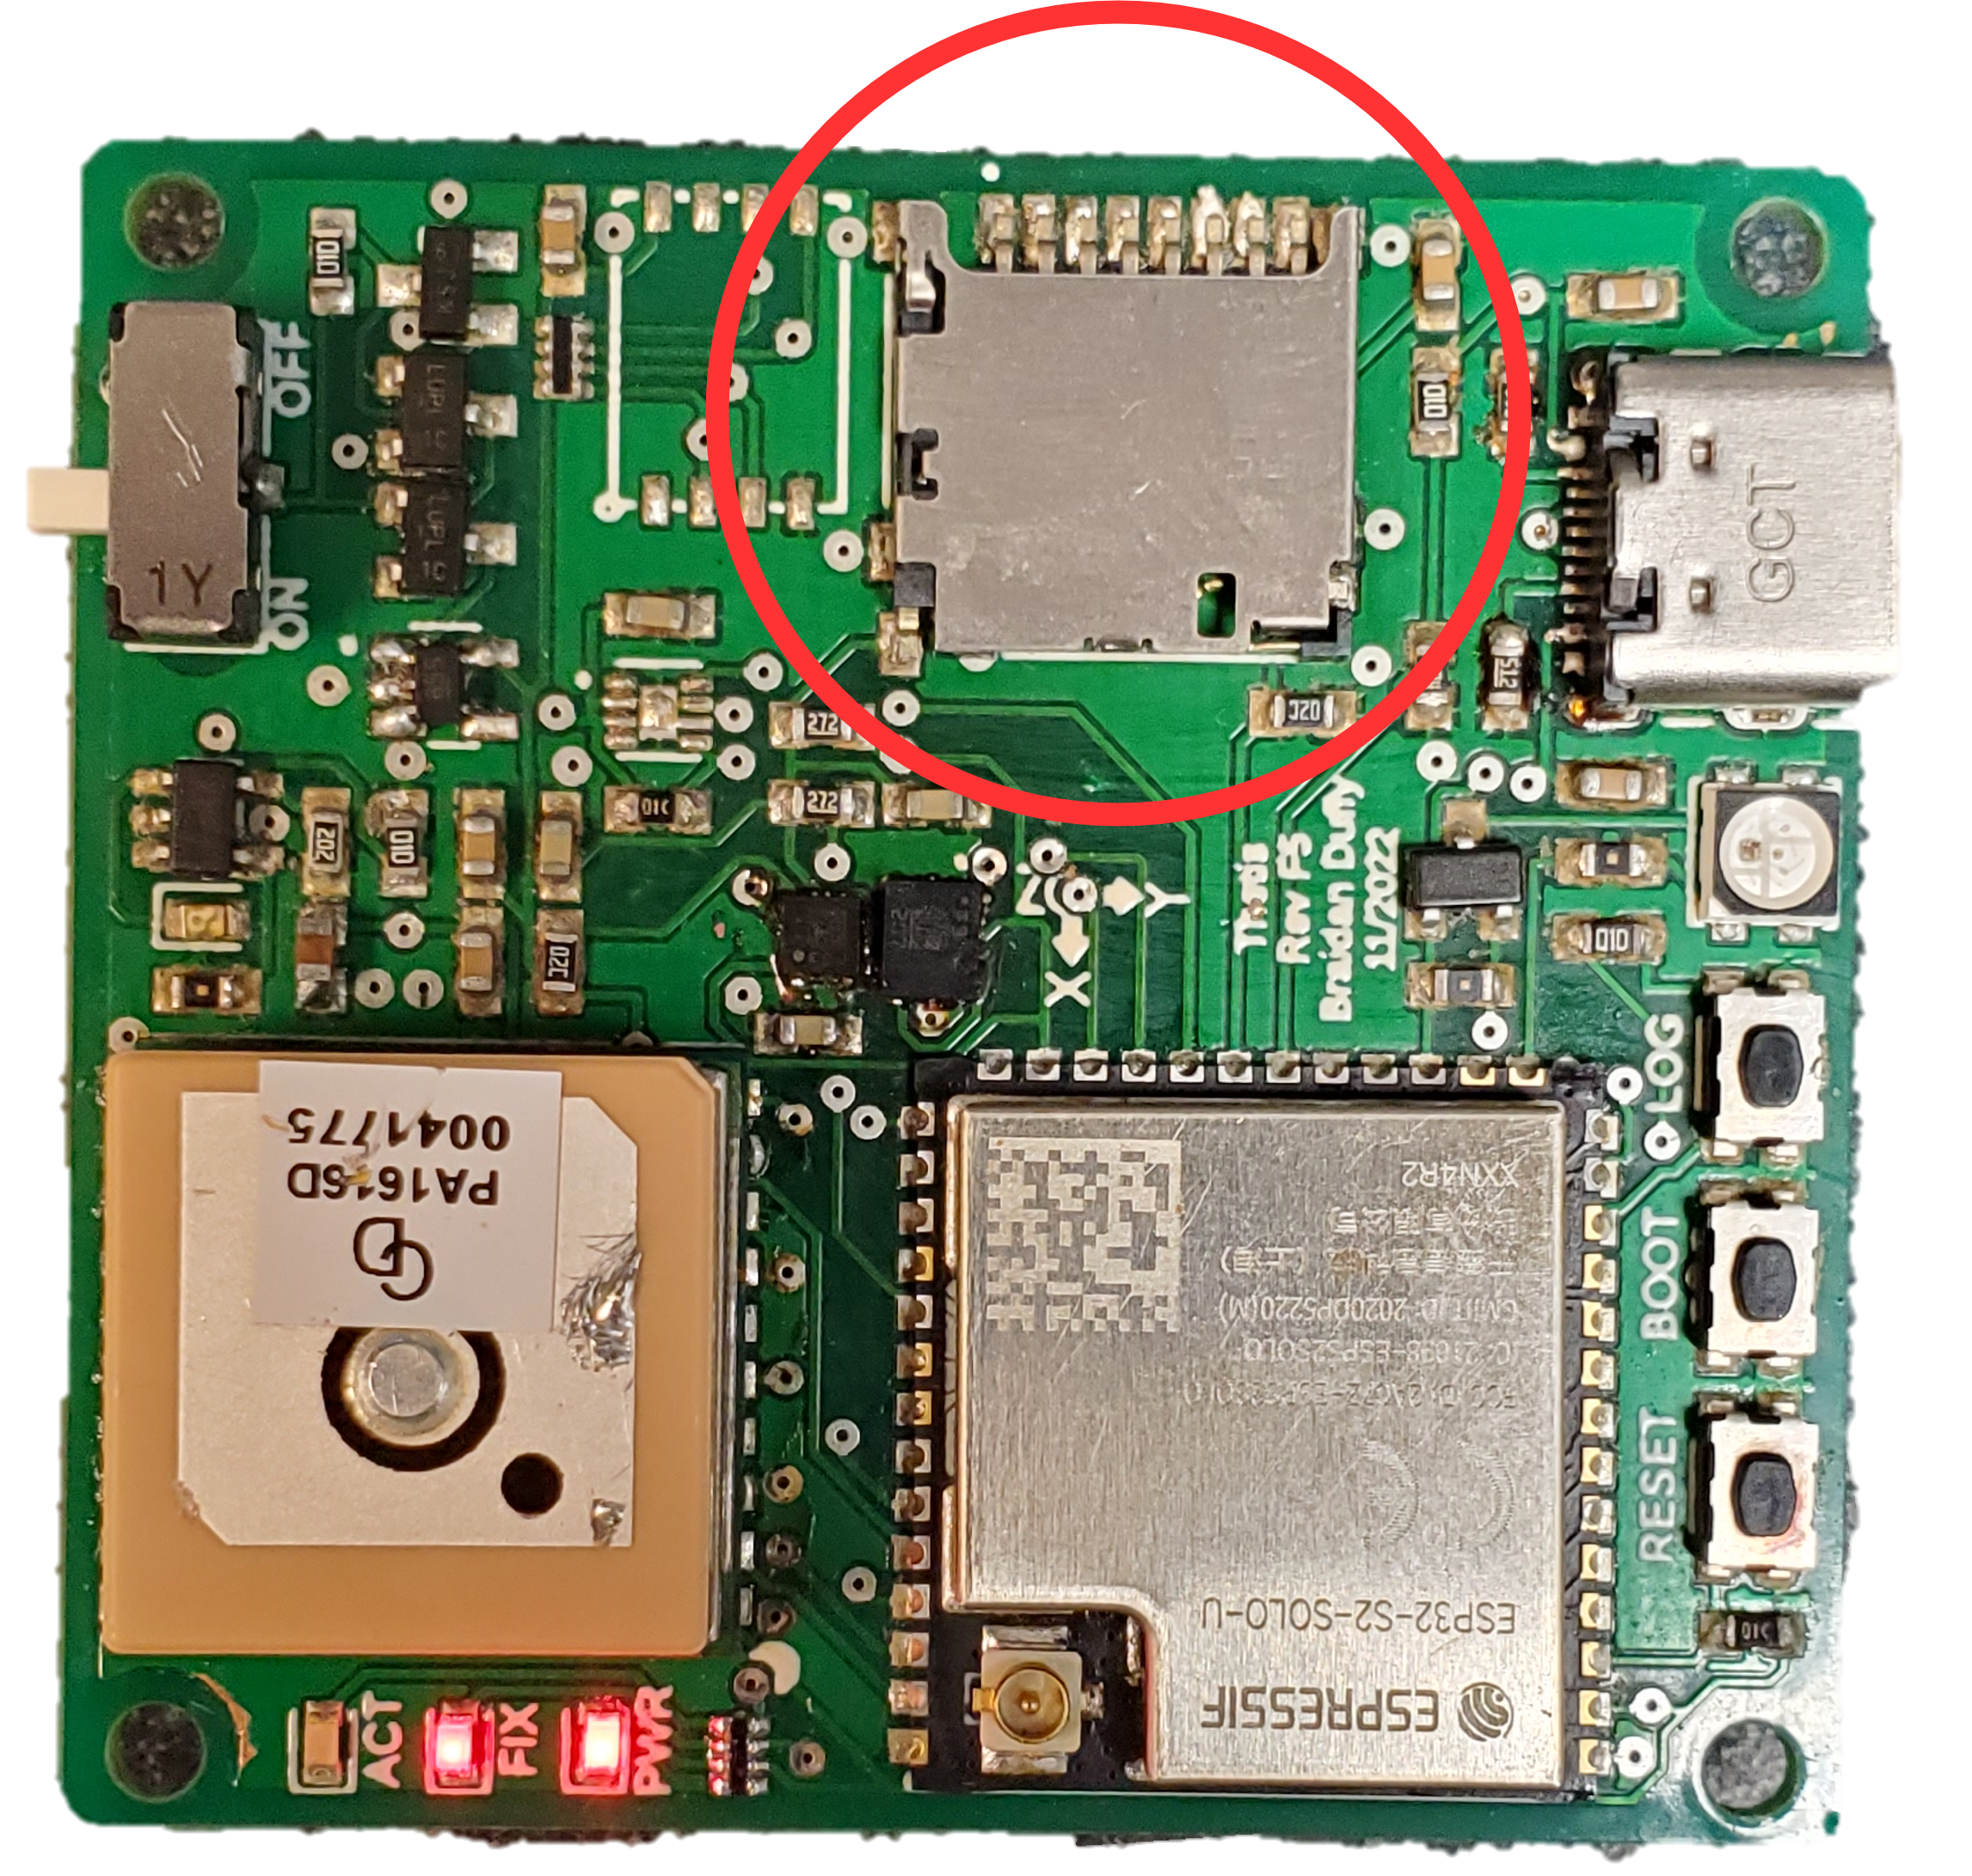
\includegraphics[width=0.5\textwidth]{troubleshooting/filesystem_error_bug.png}
    \caption{The microSD card is not present at startup, but the device does not blink an error code.}
    \label{fig:filesystem_error_bug}
\end{figure}

\subsubsection{Thetis Not Showing Up in x-IMU3 GUI}
When Thetis is connected to a host computer over USB, it will not automatically start broadcasting data or interact with the x-IMU3 GUI.
This is because the firmware is in a diagnostic state and waiting for a serial terminal to open before streaming data.
Therefore, when using Thetis with the x-IMU3 GUI, plug it in, turn on the device and open a serial monitor to it as described above.
Then, open the x-IMU3 GUI and the device should be present.

\subsubsection{The Sensors are Reporting Data, but it is all Zeros}
Sometime
    \input{sections/communication_protocol}
    \input{sections/sample_rates}
    \input{sections/network_announcement}
    \section{Device Settings}

\subsection{Individual Settings}
\label{sec:individualSettings}

% This file was generated by individual_settings.py

\begingroup
    \def\tempSection{Calibration date (read-only)}
    \def\tempLabel{sec:calibrationDate}
    \def\tempDescription
    {
        Calibration date.
    }
    \def\tempKey{calibrationDate}
    \def\tempType{string}
    \def\tempDefault{\enquote{Unknown}}
    \deviceSetting
\endgroup

\begingroup
    \def\tempSection{System clock calibration (read-only)}
    \def\tempLabel{sec:systemClockCalibration}
    \def\tempDescription
    {
        System clock calibration.
    }
    \def\tempKey{systemClockCalibration}
    \def\tempType{number}
    \def\tempDefault{1.0}
    \deviceSetting
\endgroup

\begingroup
    \def\tempSection{\acs{RTC} calibration (read-only)}
    \def\tempLabel{sec:rtcCalibration}
    \def\tempDescription
    {
        \ac{RTC} calibration.
    }
    \def\tempKey{rtcCalibration}
    \def\tempType{number}
    \def\tempDefault{1.0}
    \deviceSetting
\endgroup

\begingroup
    \def\tempSection{Battery voltmeter sensitivity (read-only)}
    \def\tempLabel{sec:batteryVoltmeterSensitivity}
    \def\tempDescription
    {
        Battery voltmeter sensitivity.
    }
    \def\tempKey{batteryVoltmeterSensitivity}
    \def\tempType{number}
    \def\tempDefault{1.0}
    \deviceSetting
\endgroup

\begingroup
    \def\tempSection{Gyroscope misalignment (read-only)}
    \def\tempLabel{sec:gyroscopeMisalignment}
    \def\tempDescription
    {
        Gyroscope misalignment.
    }
    \def\tempKey{gyroscopeMisalignment}
    \def\tempType{array of 9 numbers}
    \def\tempDefault{[1.0, 0.0, 0.0, 0.0, 1.0, 0.0, 0.0, 0.0, 1.0]}
    \deviceSetting
\endgroup

\begingroup
    \def\tempSection{Gyroscope sensitivity (read-only)}
    \def\tempLabel{sec:gyroscopeSensitivity}
    \def\tempDescription
    {
        Gyroscope sensitivity.
    }
    \def\tempKey{gyroscopeSensitivity}
    \def\tempType{array of 3 numbers}
    \def\tempDefault{[1.0, 1.0, 1.0]}
    \deviceSetting
\endgroup

\begingroup
    \def\tempSection{Gyroscope offset (read-only)}
    \def\tempLabel{sec:gyroscopeOffset}
    \def\tempDescription
    {
        Gyroscope offset.
    }
    \def\tempKey{gyroscopeOffset}
    \def\tempType{array of 3 numbers}
    \def\tempDefault{[0.0, 0.0, 0.0]}
    \deviceSetting
\endgroup

\begingroup
    \def\tempSection{Accelerometer misalignment (read-only)}
    \def\tempLabel{sec:accelerometerMisalignment}
    \def\tempDescription
    {
        Accelerometer misalignment.
    }
    \def\tempKey{accelerometerMisalignment}
    \def\tempType{array of 9 numbers}
    \def\tempDefault{[1.0, 0.0, 0.0, 0.0, 1.0, 0.0, 0.0, 0.0, 1.0]}
    \deviceSetting
\endgroup

\begingroup
    \def\tempSection{Accelerometer sensitivity (read-only)}
    \def\tempLabel{sec:accelerometerSensitivity}
    \def\tempDescription
    {
        Accelerometer sensitivity.
    }
    \def\tempKey{accelerometerSensitivity}
    \def\tempType{array of 3 numbers}
    \def\tempDefault{[1.0, 1.0, 1.0]}
    \deviceSetting
\endgroup

\begingroup
    \def\tempSection{Accelerometer offset (read-only)}
    \def\tempLabel{sec:accelerometerOffset}
    \def\tempDescription
    {
        Accelerometer offset.
    }
    \def\tempKey{accelerometerOffset}
    \def\tempType{array of 3 numbers}
    \def\tempDefault{[0.0, 0.0, 0.0]}
    \deviceSetting
\endgroup

\begingroup
    \def\tempSection{Soft iron matrix (read-only)}
    \def\tempLabel{sec:softIronMatrix}
    \def\tempDescription
    {
        Soft iron matrix.
    }
    \def\tempKey{softIronMatrix}
    \def\tempType{array of 9 numbers}
    \def\tempDefault{[1.0, 0.0, 0.0, 0.0, 1.0, 0.0, 0.0, 0.0, 1.0]}
    \deviceSetting
\endgroup

\begingroup
    \def\tempSection{Hard iron offset (read-only)}
    \def\tempLabel{sec:hardIronOffset}
    \def\tempDescription
    {
        Hard iron offset.
    }
    \def\tempKey{hardIronOffset}
    \def\tempType{array of 3 numbers}
    \def\tempDefault{[0.0, 0.0, 0.0]}
    \deviceSetting
\endgroup

\begingroup
    \def\tempSection{High-g accelerometer misalignment (read-only)}
    \def\tempLabel{sec:highGAccelerometerMisalignment}
    \def\tempDescription
    {
        High-g accelerometer misalignment.
    }
    \def\tempKey{highGAccelerometerMisalignment}
    \def\tempType{array of 9 numbers}
    \def\tempDefault{[1.0, 0.0, 0.0, 0.0, 1.0, 0.0, 0.0, 0.0, 1.0]}
    \deviceSetting
\endgroup

\begingroup
    \def\tempSection{High-g accelerometer sensitivity (read-only)}
    \def\tempLabel{sec:highGAccelerometerSensitivity}
    \def\tempDescription
    {
        High-g accelerometer sensitivity.
    }
    \def\tempKey{highGAccelerometerSensitivity}
    \def\tempType{array of 3 numbers}
    \def\tempDefault{[1.0, 1.0, 1.0]}
    \deviceSetting
\endgroup

\begingroup
    \def\tempSection{High-g accelerometer offset (read-only)}
    \def\tempLabel{sec:highGAccelerometerOffset}
    \def\tempDescription
    {
        High-g accelerometer offset.
    }
    \def\tempKey{highGAccelerometerOffset}
    \def\tempType{array of 3 numbers}
    \def\tempDefault{[0.0, 0.0, 0.0]}
    \deviceSetting
\endgroup

\begingroup
    \def\tempSection{Device name}
    \def\tempLabel{sec:deviceName}
    \def\tempDescription
    {
        Device name.
    }
    \def\tempKey{deviceName}
    \def\tempType{string}
    \def\tempDefault{\enquote{x-IMU3}}
    \deviceSetting
\endgroup

\begingroup
    \def\tempSection{Serial number (read-only)}
    \def\tempLabel{sec:serialNumber}
    \def\tempDescription
    {
        Serial number.
    }
    \def\tempKey{serialNumber}
    \def\tempType{string}
    \def\tempDefault{\enquote{Unknown}}
    \deviceSetting
\endgroup

\begingroup
    \def\tempSection{Firmware version (read-only)}
    \def\tempLabel{sec:firmwareVersion}
    \def\tempDescription
    {
        Firmware version.
    }
    \def\tempKey{firmwareVersion}
    \def\tempType{string}
    \def\tempDefault{\enquote{Unknown}}
    \deviceSetting
\endgroup

\begingroup
    \def\tempSection{Bootloader version (read-only)}
    \def\tempLabel{sec:bootloaderVersion}
    \def\tempDescription
    {
        Bootloader version.
    }
    \def\tempKey{bootloaderVersion}
    \def\tempType{string}
    \def\tempDefault{\enquote{Unknown}}
    \deviceSetting
\endgroup

\begingroup
    \def\tempSection{Hardware version (read-only)}
    \def\tempLabel{sec:hardwareVersion}
    \def\tempDescription
    {
        Hardware version.
    }
    \def\tempKey{hardwareVersion}
    \def\tempType{string}
    \def\tempDefault{\enquote{Unknown}}
    \deviceSetting
\endgroup

\begingroup
    \def\tempSection{Serial mode}
    \def\tempLabel{sec:serialMode}
    \def\tempDescription
    {
        Serial mode.
    }
    \def\tempKey{serialMode}
    \def\tempType{number}
    \def\tempDefault{0}
    \deviceSetting
\endgroup

\begingroup
    \def\tempSection{Serial baud rate}
    \def\tempLabel{sec:serialBaudRate}
    \def\tempDescription
    {
        Serial baud rate.
    }
    \def\tempKey{serialBaudRate}
    \def\tempType{number}
    \def\tempDefault{115200}
    \deviceSetting
\endgroup

\begingroup
    \def\tempSection{Serial \acs{RTS}/\acs{CTS} enabled}
    \def\tempLabel{sec:serialRtsCtsEnabled}
    \def\tempDescription
    {
        Serial \ac{RTS}/\ac{CTS} enabled.
    }
    \def\tempKey{serialRtsCtsEnabled}
    \def\tempType{true or false}
    \def\tempDefault{false}
    \deviceSetting
\endgroup

\begingroup
    \def\tempSection{Serial accessory number of bytes}
    \def\tempLabel{sec:serialAccessoryNumberOfBytes}
    \def\tempDescription
    {
        Serial accessory number of bytes.
    }
    \def\tempKey{serialAccessoryNumberOfBytes}
    \def\tempType{number}
    \def\tempDefault{1024}
    \deviceSetting
\endgroup

\begingroup
    \def\tempSection{Serial accessory termination byte}
    \def\tempLabel{sec:serialAccessoryTerminationByte}
    \def\tempDescription
    {
        Serial accessory termination byte.
    }
    \def\tempKey{serialAccessoryTerminationByte}
    \def\tempType{number}
    \def\tempDefault{10}
    \deviceSetting
\endgroup

\begingroup
    \def\tempSection{Serial accessory timeout}
    \def\tempLabel{sec:serialAccessoryTimeout}
    \def\tempDescription
    {
        Serial accessory timeout.
    }
    \def\tempKey{serialAccessoryTimeout}
    \def\tempType{number}
    \def\tempDefault{100}
    \deviceSetting
\endgroup

\begingroup
    \def\tempSection{Wireless mode}
    \def\tempLabel{sec:wirelessMode}
    \def\tempDescription
    {
        Wireless mode.
    }
    \def\tempKey{wirelessMode}
    \def\tempType{number}
    \def\tempDefault{2}
    \deviceSetting
\endgroup

\begingroup
    \def\tempSection{Wireless firmware version (read-only)}
    \def\tempLabel{sec:wirelessFirmwareVersion}
    \def\tempDescription
    {
        Wireless firmware version.
    }
    \def\tempKey{wirelessFirmwareVersion}
    \def\tempType{string}
    \def\tempDefault{\enquote{Unknown}}
    \deviceSetting
\endgroup

\begingroup
    \def\tempSection{External antennae enabled}
    \def\tempLabel{sec:externalAntennaeEnabled}
    \def\tempDescription
    {
        External antennae enabled.
    }
    \def\tempKey{externalAntennaeEnabled}
    \def\tempType{true or false}
    \def\tempDefault{false}
    \deviceSetting
\endgroup

\begingroup
    \def\tempSection{Wi-Fi region}
    \def\tempLabel{sec:wiFiRegion}
    \def\tempDescription
    {
        Wi-Fi region.
    }
    \def\tempKey{wiFiRegion}
    \def\tempType{number}
    \def\tempDefault{2}
    \deviceSetting
\endgroup

\begingroup
    \def\tempSection{Wi-Fi \acs{MAC} address (read-only)}
    \def\tempLabel{sec:wiFiMacAddress}
    \def\tempDescription
    {
        Wi-Fi \ac{MAC} address.
    }
    \def\tempKey{wiFiMacAddress}
    \def\tempType{string}
    \def\tempDefault{0}
    \deviceSetting
\endgroup

\begingroup
    \def\tempSection{Wi-Fi \acs{IP} address (read-only)}
    \def\tempLabel{sec:wiFiIPAddress}
    \def\tempDescription
    {
        Wi-Fi \ac{IP} address.
    }
    \def\tempKey{wiFiIPAddress}
    \def\tempType{string}
    \def\tempDefault{0}
    \deviceSetting
\endgroup

\begingroup
    \def\tempSection{Wi-Fi client \acs{SSID}}
    \def\tempLabel{sec:wiFiClientSsid}
    \def\tempDescription
    {
        Wi-Fi client \ac{SSID}.
    }
    \def\tempKey{wiFiClientSsid}
    \def\tempType{string}
    \def\tempDefault{\enquote{}}
    \deviceSetting
\endgroup

\begingroup
    \def\tempSection{Wi-Fi client key}
    \def\tempLabel{sec:wiFiClientKey}
    \def\tempDescription
    {
        Wi-Fi client key.
    }
    \def\tempKey{wiFiClientKey}
    \def\tempType{string}
    \def\tempDefault{\enquote{}}
    \deviceSetting
\endgroup

\begingroup
    \def\tempSection{Wi-Fi client channel}
    \def\tempLabel{sec:wiFiClientChannel}
    \def\tempDescription
    {
        Wi-Fi client channel.
    }
    \def\tempKey{wiFiClientChannel}
    \def\tempType{number}
    \def\tempDefault{0}
    \deviceSetting
\endgroup

\begingroup
    \def\tempSection{Wi-Fi client \acs{DHCP} enabled}
    \def\tempLabel{sec:wiFiClientDhcpEnabled}
    \def\tempDescription
    {
        Wi-Fi client \ac{DHCP} enabled.
    }
    \def\tempKey{wiFiClientDhcpEnabled}
    \def\tempType{true or false}
    \def\tempDefault{true}
    \deviceSetting
\endgroup

\begingroup
    \def\tempSection{Wi-Fi client \acs{IP} address}
    \def\tempLabel{sec:wiFiClientIPAddress}
    \def\tempDescription
    {
        Wi-Fi client \ac{IP} address.
    }
    \def\tempKey{wiFiClientIPAddress}
    \def\tempType{string}
    \def\tempDefault{\enquote{192.168.1.2}}
    \deviceSetting
\endgroup

\begingroup
    \def\tempSection{Wi-Fi client netmask}
    \def\tempLabel{sec:wiFiClientNetmask}
    \def\tempDescription
    {
        Wi-Fi client netmask.
    }
    \def\tempKey{wiFiClientNetmask}
    \def\tempType{string}
    \def\tempDefault{\enquote{255.255.255.0}}
    \deviceSetting
\endgroup

\begingroup
    \def\tempSection{Wi-Fi client gateway}
    \def\tempLabel{sec:wiFiClientGateway}
    \def\tempDescription
    {
        Wi-Fi client gateway.
    }
    \def\tempKey{wiFiClientGateway}
    \def\tempType{string}
    \def\tempDefault{\enquote{192.168.1.1}}
    \deviceSetting
\endgroup

\begingroup
    \def\tempSection{Wi-Fi \acs{AP} \acs{SSID}}
    \def\tempLabel{sec:wiFiAPSsid}
    \def\tempDescription
    {
        Wi-Fi \ac{AP} \ac{SSID}.
    }
    \def\tempKey{wiFiAPSsid}
    \def\tempType{string}
    \def\tempDefault{\enquote{}}
    \deviceSetting
\endgroup

\begingroup
    \def\tempSection{Wi-Fi \acs{AP} key}
    \def\tempLabel{sec:wiFiAPKey}
    \def\tempDescription
    {
        Wi-Fi \ac{AP} key.
    }
    \def\tempKey{wiFiAPKey}
    \def\tempType{string}
    \def\tempDefault{\enquote{}}
    \deviceSetting
\endgroup

\begingroup
    \def\tempSection{Wi-Fi \acs{AP} channel}
    \def\tempLabel{sec:wiFiAPChannel}
    \def\tempDescription
    {
        Wi-Fi \ac{AP} channel.
    }
    \def\tempKey{wiFiAPChannel}
    \def\tempType{number}
    \def\tempDefault{36}
    \deviceSetting
\endgroup

\begingroup
    \def\tempSection{Wi-Fi \acs{AP} \acs{IP} address}
    \def\tempLabel{sec:wiFiAPIPAddress}
    \def\tempDescription
    {
        Wi-Fi \ac{AP} \ac{IP} address.
    }
    \def\tempKey{wiFiAPIPAddress}
    \def\tempType{string}
    \def\tempDefault{0x0101A9C0}
    \deviceSetting
\endgroup

\begingroup
    \def\tempSection{\acs{TCP} port}
    \def\tempLabel{sec:tcpPort}
    \def\tempDescription
    {
        \ac{TCP} port.
    }
    \def\tempKey{tcpPort}
    \def\tempType{number}
    \def\tempDefault{7000}
    \deviceSetting
\endgroup

\begingroup
    \def\tempSection{\acs{UDP} \acs{IP} address}
    \def\tempLabel{sec:udpIPAddress}
    \def\tempDescription
    {
        \ac{UDP} \ac{IP} address.
    }
    \def\tempKey{udpIPAddress}
    \def\tempType{string}
    \def\tempDefault{0}
    \deviceSetting
\endgroup

\begingroup
    \def\tempSection{\acs{UDP} send port}
    \def\tempLabel{sec:udpSendPort}
    \def\tempDescription
    {
        \ac{UDP} send port.
    }
    \def\tempKey{udpSendPort}
    \def\tempType{number}
    \def\tempDefault{0}
    \deviceSetting
\endgroup

\begingroup
    \def\tempSection{\acs{UDP} receive port}
    \def\tempLabel{sec:udpReceivePort}
    \def\tempDescription
    {
        \ac{UDP} receive port.
    }
    \def\tempKey{udpReceivePort}
    \def\tempType{number}
    \def\tempDefault{9000}
    \deviceSetting
\endgroup

\begingroup
    \def\tempSection{\acs{UDP} low latency}
    \def\tempLabel{sec:udpLowLatency}
    \def\tempDescription
    {
        \ac{UDP} low latency.
    }
    \def\tempKey{udpLowLatency}
    \def\tempType{true or false}
    \def\tempDefault{false}
    \deviceSetting
\endgroup

\begingroup
    \def\tempSection{Synchronisation enabled}
    \def\tempLabel{sec:synchronisationEnabled}
    \def\tempDescription
    {
        Synchronisation enabled.
    }
    \def\tempKey{synchronisationEnabled}
    \def\tempType{true or false}
    \def\tempDefault{true}
    \deviceSetting
\endgroup

\begingroup
    \def\tempSection{Synchronisation network latency}
    \def\tempLabel{sec:synchronisationNetworkLatency}
    \def\tempDescription
    {
        Synchronisation network latency.
    }
    \def\tempKey{synchronisationNetworkLatency}
    \def\tempType{number}
    \def\tempDefault{1500}
    \deviceSetting
\endgroup

\begingroup
    \def\tempSection{Bluetooth address (read-only)}
    \def\tempLabel{sec:bluetoothAddress}
    \def\tempDescription
    {
        Bluetooth address.
    }
    \def\tempKey{bluetoothAddress}
    \def\tempType{number}
    \def\tempDefault{0}
    \deviceSetting
\endgroup

\begingroup
    \def\tempSection{Bluetooth name}
    \def\tempLabel{sec:bluetoothName}
    \def\tempDescription
    {
        Bluetooth name.
    }
    \def\tempKey{bluetoothName}
    \def\tempType{string}
    \def\tempDefault{\enquote{}}
    \deviceSetting
\endgroup

\begingroup
    \def\tempSection{Bluetooth pin code}
    \def\tempLabel{sec:bluetoothPinCode}
    \def\tempDescription
    {
        Bluetooth pin code.
    }
    \def\tempKey{bluetoothPinCode}
    \def\tempType{string}
    \def\tempDefault{\enquote{}}
    \deviceSetting
\endgroup

\begingroup
    \def\tempSection{Bluetooth discovery mode}
    \def\tempLabel{sec:bluetoothDiscoveryMode}
    \def\tempDescription
    {
        Bluetooth discovery mode.
    }
    \def\tempKey{bluetoothDiscoveryMode}
    \def\tempType{number}
    \def\tempDefault{2}
    \deviceSetting
\endgroup

\begingroup
    \def\tempSection{Bluetooth paired address (read-only)}
    \def\tempLabel{sec:bluetoothPairedAddress}
    \def\tempDescription
    {
        Bluetooth paired address.
    }
    \def\tempKey{bluetoothPairedAddress}
    \def\tempType{number}
    \def\tempDefault{0}
    \deviceSetting
\endgroup

\begingroup
    \def\tempSection{Bluetooth paired link key (read-only)}
    \def\tempLabel{sec:bluetoothPairedLinkKey}
    \def\tempDescription
    {
        Bluetooth paired link key.
    }
    \def\tempKey{bluetoothPairedLinkKey}
    \def\tempType{number}
    \def\tempDefault{0}
    \deviceSetting
\endgroup

\begingroup
    \def\tempSection{Data logger enabled}
    \def\tempLabel{sec:dataLoggerEnabled}
    \def\tempDescription
    {
        Data logger enabled.
    }
    \def\tempKey{dataLoggerEnabled}
    \def\tempType{true or false}
    \def\tempDefault{false}
    \deviceSetting
\endgroup

\begingroup
    \def\tempSection{Data logger file name prefix}
    \def\tempLabel{sec:dataLoggerFileNamePrefix}
    \def\tempDescription
    {
        Data logger file name prefix.
    }
    \def\tempKey{dataLoggerFileNamePrefix}
    \def\tempType{string}
    \def\tempDefault{\enquote{}}
    \deviceSetting
\endgroup

\begingroup
    \def\tempSection{Data logger file name time enabled}
    \def\tempLabel{sec:dataLoggerFileNameTimeEnabled}
    \def\tempDescription
    {
        Data logger file name time enabled.
    }
    \def\tempKey{dataLoggerFileNameTimeEnabled}
    \def\tempType{true or false}
    \def\tempDefault{true}
    \deviceSetting
\endgroup

\begingroup
    \def\tempSection{Data logger file name counter enabled}
    \def\tempLabel{sec:dataLoggerFileNameCounterEnabled}
    \def\tempDescription
    {
        Data logger file name counter enabled.
    }
    \def\tempKey{dataLoggerFileNameCounterEnabled}
    \def\tempType{true or false}
    \def\tempDefault{false}
    \deviceSetting
\endgroup

\begingroup
    \def\tempSection{Data logger max file size}
    \def\tempLabel{sec:dataLoggerMaxFileSize}
    \def\tempDescription
    {
        Data logger max file size.
    }
    \def\tempKey{dataLoggerMaxFileSize}
    \def\tempType{number}
    \def\tempDefault{0}
    \deviceSetting
\endgroup

\begingroup
    \def\tempSection{Data logger max file period}
    \def\tempLabel{sec:dataLoggerMaxFilePeriod}
    \def\tempDescription
    {
        Data logger max file period.
    }
    \def\tempKey{dataLoggerMaxFilePeriod}
    \def\tempType{number}
    \def\tempDefault{0}
    \deviceSetting
\endgroup

\begingroup
    \def\tempSection{Axes alignment}
    \def\tempLabel{sec:axesAlignment}
    \def\tempDescription
    {
        Axes alignment.
    }
    \def\tempKey{axesAlignment}
    \def\tempType{number}
    \def\tempDefault{0}
    \deviceSetting
\endgroup

\begingroup
    \def\tempSection{Gyroscope offset correction enabled}
    \def\tempLabel{sec:gyroscopeOffsetCorrectionEnabled}
    \def\tempDescription
    {
        Gyroscope offset correction enabled.
    }
    \def\tempKey{gyroscopeOffsetCorrectionEnabled}
    \def\tempType{true or false}
    \def\tempDefault{true}
    \deviceSetting
\endgroup

\begingroup
    \def\tempSection{\acs{AHRS} axes convention}
    \def\tempLabel{sec:ahrsAxesConvention}
    \def\tempDescription
    {
        \ac{AHRS} axes convention.
    }
    \def\tempKey{ahrsAxesConvention}
    \def\tempType{number}
    \def\tempDefault{0}
    \deviceSetting
\endgroup

\begingroup
    \def\tempSection{\acs{AHRS} gain}
    \def\tempLabel{sec:ahrsGain}
    \def\tempDescription
    {
        \ac{AHRS} gain.
    }
    \def\tempKey{ahrsGain}
    \def\tempType{number}
    \def\tempDefault{0.5}
    \deviceSetting
\endgroup

\begingroup
    \def\tempSection{\acs{AHRS} ignore magnetometer}
    \def\tempLabel{sec:ahrsIgnoreMagnetometer}
    \def\tempDescription
    {
        \ac{AHRS} ignore magnetometer.
    }
    \def\tempKey{ahrsIgnoreMagnetometer}
    \def\tempType{true or false}
    \def\tempDefault{false}
    \deviceSetting
\endgroup

\begingroup
    \def\tempSection{\acs{AHRS} acceleration rejection enabled}
    \def\tempLabel{sec:ahrsAccelerationRejectionEnabled}
    \def\tempDescription
    {
        \ac{AHRS} acceleration rejection enabled.
    }
    \def\tempKey{ahrsAccelerationRejectionEnabled}
    \def\tempType{true or false}
    \def\tempDefault{true}
    \deviceSetting
\endgroup

\begingroup
    \def\tempSection{\acs{AHRS} magnetic rejection enabled}
    \def\tempLabel{sec:ahrsMagneticRejectionEnabled}
    \def\tempDescription
    {
        \ac{AHRS} magnetic rejection enabled.
    }
    \def\tempKey{ahrsMagneticRejectionEnabled}
    \def\tempType{true or false}
    \def\tempDefault{true}
    \deviceSetting
\endgroup

\begingroup
    \def\tempSection{Binary mode enabled}
    \def\tempLabel{sec:binaryModeEnabled}
    \def\tempDescription
    {
        Binary mode enabled.
    }
    \def\tempKey{binaryModeEnabled}
    \def\tempType{true or false}
    \def\tempDefault{true}
    \deviceSetting
\endgroup

\begingroup
    \def\tempSection{\acs{USB} data messages enabled}
    \def\tempLabel{sec:usbDataMessagesEnabled}
    \def\tempDescription
    {
        \ac{USB} data messages enabled.
    }
    \def\tempKey{usbDataMessagesEnabled}
    \def\tempType{true or false}
    \def\tempDefault{true}
    \deviceSetting
\endgroup

\begingroup
    \def\tempSection{Serial data messages enabled}
    \def\tempLabel{sec:serialDataMessagesEnabled}
    \def\tempDescription
    {
        Serial data messages enabled.
    }
    \def\tempKey{serialDataMessagesEnabled}
    \def\tempType{true or false}
    \def\tempDefault{true}
    \deviceSetting
\endgroup

\begingroup
    \def\tempSection{\acs{TCP} data messages enabled}
    \def\tempLabel{sec:tcpDataMessagesEnabled}
    \def\tempDescription
    {
        \ac{TCP} data messages enabled.
    }
    \def\tempKey{tcpDataMessagesEnabled}
    \def\tempType{true or false}
    \def\tempDefault{true}
    \deviceSetting
\endgroup

\begingroup
    \def\tempSection{\acs{UDP} data messages enabled}
    \def\tempLabel{sec:udpDataMessagesEnabled}
    \def\tempDescription
    {
        \ac{UDP} data messages enabled.
    }
    \def\tempKey{udpDataMessagesEnabled}
    \def\tempType{true or false}
    \def\tempDefault{true}
    \deviceSetting
\endgroup

\begingroup
    \def\tempSection{Bluetooth data messages enabled}
    \def\tempLabel{sec:bluetoothDataMessagesEnabled}
    \def\tempDescription
    {
        Bluetooth data messages enabled.
    }
    \def\tempKey{bluetoothDataMessagesEnabled}
    \def\tempType{true or false}
    \def\tempDefault{true}
    \deviceSetting
\endgroup

\begingroup
    \def\tempSection{Data logger data messages enabled}
    \def\tempLabel{sec:dataLoggerDataMessagesEnabled}
    \def\tempDescription
    {
        Data logger data messages enabled.
    }
    \def\tempKey{dataLoggerDataMessagesEnabled}
    \def\tempType{true or false}
    \def\tempDefault{true}
    \deviceSetting
\endgroup

\begingroup
    \def\tempSection{\acs{AHRS} message type}
    \def\tempLabel{sec:ahrsMessageType}
    \def\tempDescription
    {
        \ac{AHRS} message type.
    }
    \def\tempKey{ahrsMessageType}
    \def\tempType{number}
    \def\tempDefault{0}
    \deviceSetting
\endgroup

\begingroup
    \def\tempSection{Inertial message rate divisor}
    \def\tempLabel{sec:inertialMessageRateDivisor}
    \def\tempDescription
    {
        Inertial message rate divisor.
    }
    \def\tempKey{inertialMessageRateDivisor}
    \def\tempType{number}
    \def\tempDefault{8}
    \deviceSetting
\endgroup

\begingroup
    \def\tempSection{Magnetometer message rate divisor}
    \def\tempLabel{sec:magnetometerMessageRateDivisor}
    \def\tempDescription
    {
        Magnetometer message rate divisor.
    }
    \def\tempKey{magnetometerMessageRateDivisor}
    \def\tempType{number}
    \def\tempDefault{1}
    \deviceSetting
\endgroup

\begingroup
    \def\tempSection{\acs{AHRS} message rate divisor}
    \def\tempLabel{sec:ahrsMessageRateDivisor}
    \def\tempDescription
    {
        \ac{AHRS} message rate divisor.
    }
    \def\tempKey{ahrsMessageRateDivisor}
    \def\tempType{number}
    \def\tempDefault{8}
    \deviceSetting
\endgroup

\begingroup
    \def\tempSection{High-g accelerometer message rate divisor}
    \def\tempLabel{sec:highGAccelerometerMessageRateDivisor}
    \def\tempDescription
    {
        High-g accelerometer message rate divisor.
    }
    \def\tempKey{highGAccelerometerMessageRateDivisor}
    \def\tempType{number}
    \def\tempDefault{32}
    \deviceSetting
\endgroup

\begingroup
    \def\tempSection{Temperature message rate divisor}
    \def\tempLabel{sec:temperatureMessageRateDivisor}
    \def\tempDescription
    {
        Temperature message rate divisor.
    }
    \def\tempKey{temperatureMessageRateDivisor}
    \def\tempType{number}
    \def\tempDefault{5}
    \deviceSetting
\endgroup

\begingroup
    \def\tempSection{Battery message rate divisor}
    \def\tempLabel{sec:batteryMessageRateDivisor}
    \def\tempDescription
    {
        Battery message rate divisor.
    }
    \def\tempKey{batteryMessageRateDivisor}
    \def\tempType{number}
    \def\tempDefault{5}
    \deviceSetting
\endgroup

\begingroup
    \def\tempSection{\acs{RSSI} message rate divisor}
    \def\tempLabel{sec:rssiMessageRateDivisor}
    \def\tempDescription
    {
        \ac{RSSI} message rate divisor.
    }
    \def\tempKey{rssiMessageRateDivisor}
    \def\tempType{number}
    \def\tempDefault{1}
    \deviceSetting
\endgroup

\begingroup
    \def\tempSection{\acs{FTP} enabled}
    \def\tempLabel{sec:ftpEnabled}
    \def\tempDescription
    {
        \ac{FTP} enabled.
    }
    \def\tempKey{ftpEnabled}
    \def\tempType{true or false}
    \def\tempDefault{false}
    \deviceSetting
\endgroup

\begingroup
    \def\tempSection{\acs{FTP} username}
    \def\tempLabel{sec:ftpUsername}
    \def\tempDescription
    {
        \ac{FTP} username.
    }
    \def\tempKey{ftpUsername}
    \def\tempType{string}
    \def\tempDefault{\enquote{}}
    \deviceSetting
\endgroup

\begingroup
    \def\tempSection{Log print level}
    \def\tempLabel{sec:logPrintLevel}
    \def\tempDescription
    {
        Log print level.
    }
    \def\tempKey{logPrintLevel}
    \def\tempType{number}
    \def\tempDefault{0}
    \deviceSetting
\endgroup

\begingroup
    \def\tempSection{Log file level}
    \def\tempLabel{sec:logFileLevel}
    \def\tempDescription
    {
        Log file level.
    }
    \def\tempKey{logFileLevel}
    \def\tempType{number}
    \def\tempDefault{2}
    \deviceSetting
\endgroup

\begingroup
    \def\tempSection{\acs{GPS} \acs{RTC} sync enabled}
    \def\tempLabel{sec:gpsRtcSyncEnabled}
    \def\tempDescription
    {
        \ac{GPS} \ac{RTC} sync enabled.
    }
    \def\tempKey{gpsRtcSyncEnabled}
    \def\tempType{true or false}
    \def\tempDefault{false}
    \deviceSetting
\endgroup

\begingroup
    \def\tempSection{Accelerometer range}
    \def\tempLabel{sec:accelerometerRange}
    \def\tempDescription
    {
        Accelerometer range.
    }
    \def\tempKey{accelerometerRange}
    \def\tempType{number}
    \def\tempDefault{2}
    \deviceSetting
\endgroup

\begingroup
    \def\tempSection{Gyroscope range}
    \def\tempLabel{sec:gyroscopeRange}
    \def\tempDescription
    {
        Gyroscope range.
    }
    \def\tempKey{gyroscopeRange}
    \def\tempType{number}
    \def\tempDefault{0}
    \deviceSetting
\endgroup

\begingroup
    \def\tempSection{\acs{IMU} data rate}
    \def\tempLabel{sec:imuDataRate}
    \def\tempDescription
    {
        \ac{IMU} data rate.
    }
    \def\tempKey{imuDataRate}
    \def\tempType{number}
    \def\tempDefault{5}
    \deviceSetting
\endgroup

\begingroup
    \def\tempSection{Magnetometer performance mode}
    \def\tempLabel{sec:magnetometerPerformanceMode}
    \def\tempDescription
    {
        Magnetometer performance mode.
    }
    \def\tempKey{magnetometerPerformanceMode}
    \def\tempType{number}
    \def\tempDefault{1}
    \deviceSetting
\endgroup

\begingroup
    \def\tempSection{Magnetometer operation mode}
    \def\tempLabel{sec:magnetometerOperationMode}
    \def\tempDescription
    {
        Magnetometer operation mode.
    }
    \def\tempKey{magnetometerOperationMode}
    \def\tempType{number}
    \def\tempDefault{0}
    \deviceSetting
\endgroup

\begingroup
    \def\tempSection{Magnetometer data rate}
    \def\tempLabel{sec:magnetometerDataRate}
    \def\tempDescription
    {
        Magnetometer data rate.
    }
    \def\tempKey{magnetometerDataRate}
    \def\tempType{number}
    \def\tempDefault{1}
    \deviceSetting
\endgroup

\begingroup
    \def\tempSection{Magnetometer range}
    \def\tempLabel{sec:magnetometerRange}
    \def\tempDescription
    {
        Magnetometer range.
    }
    \def\tempKey{magnetometerRange}
    \def\tempType{number}
    \def\tempDefault{0}
    \deviceSetting
\endgroup

\begingroup
    \def\tempSection{Gauge reset voltage}
    \def\tempLabel{sec:gaugeResetVoltage}
    \def\tempDescription
    {
        Gauge reset voltage.
    }
    \def\tempKey{gaugeResetVoltage}
    \def\tempType{number}
    \def\tempDefault{2.5}
    \deviceSetting
\endgroup

\begingroup
    \def\tempSection{Gauge activity threshold}
    \def\tempLabel{sec:gaugeActivityThreshold}
    \def\tempDescription
    {
        Gauge activity threshold.
    }
    \def\tempKey{gaugeActivityThreshold}
    \def\tempType{number}
    \def\tempDefault{0.15}
    \deviceSetting
\endgroup

\begingroup
    \def\tempSection{Gauge hibernation threshold}
    \def\tempLabel{sec:gaugeHibernationThreshold}
    \def\tempDescription
    {
        Gauge hibernation threshold.
    }
    \def\tempKey{gaugeHibernationThreshold}
    \def\tempType{number}
    \def\tempDefault{0.1}
    \deviceSetting
\endgroup

\begingroup
    \def\tempSection{Gauge alert minimum voltage}
    \def\tempLabel{sec:gaugeAlertMinimumVoltage}
    \def\tempDescription
    {
        Gauge alert minimum voltage.
    }
    \def\tempKey{gaugeAlertMinimumVoltage}
    \def\tempType{number}
    \def\tempDefault{3.0}
    \deviceSetting
\endgroup

\begingroup
    \def\tempSection{Gauge alert maximum voltage}
    \def\tempLabel{sec:gaugeAlertMaximumVoltage}
    \def\tempDescription
    {
        Gauge alert maximum voltage.
    }
    \def\tempKey{gaugeAlertMaximumVoltage}
    \def\tempType{number}
    \def\tempDefault{4.2}
    \deviceSetting
\endgroup

\begingroup
    \def\tempSection{Fusion update rate}
    \def\tempLabel{sec:fusionUpdateRate}
    \def\tempDescription
    {
        Fusion update rate.
    }
    \def\tempKey{fusionUpdateRate}
    \def\tempType{number}
    \def\tempDefault{20}
    \deviceSetting
\endgroup



    \clearpage
    \unnumberedSection{Glossary}

\begin{acronym}
    \acro{a.u.}{arbitrary units}
    \acro{ADC}{Analog-to-Digital Converter}
    \acro{AHRS}{Attitude Heading Reference System}
    \acro{AP}{Access Point}
    \acro{API}{Application Programming Interface}
    \acro{ASCII}{American Standard Code for Information Interchange}
    \acro{CDC}{Communications Device Class}
    \acro{CS}{Chip Select}
    \acro{CSV}{Comma-Separated Values}
    \acro{CTS}{Clear To Send}
    \acro{DFS}{Dynamic Frequency Selection}
    \acro{DOF}{Degree of Freedom}
    \acro{DHCP}{Dynamic Host Configuration Protocol}
    \acro{EU}{Europe}
    \acro{EEPROM}{Electrically Erasable Programmable Read-Only Memory}
    \acro{FAT32}{32-bit File Allocation Table}
    \acro{GPIO}{General Purpose Input Output}
    \acro{GPS}{Global Positioning System}
    \acro{GUI}{Graphical User Interface}
    \acro{HTTP}{Hypertext Transfer Protocol}
    \acro{I2C}{Inter-Integrated Circuit}
    \acro{IMU}{Inertial Measurement Unit}
    \acro{IP}{Internet Protocol}
    \acro{IP67}{Ingress Protection 67}
    \acro{JP}{Japan}
    \acro{JSON}{JavaScript Object Notation}
    \acro{LED}{Light-Emitting Diode}
    \acro{LF}{Line Feed}
    \acro{MAC}{Media Access Control}
    \acro{MISO}{Master In Slave Out}
    \acro{MOSI}{Master Out Slave In}
    \acro{PDF}{Portable Document Format}
    \acro{QR}{Quick Response}
    \acro{RGB}{Red Green Blue}
    \acro{RMS}{Root Mean Square}
    \acro{RSSI}{Received Signal Strength Indicator}
    \acro{RTC}{Real-Time Clock}
    \acro{RTS}{Request To Send}
    \acro{RX}{Receive}
    \acro{microSD}{micro Secure Digital}\newacroplural{microSD}[microSDs]{micro Secure Digital cards}
    \acro{SCK}{Signal Clock (SPI)}
    \acro{SCL}{Signal Clock (I2C)}
    \acro{SDA}{Signal Data}
    \acro{SLIP}{Serial Line Internet Protocol}
    \acro{SPI}{Serial Peripheral Interface}
    \acro{SPP}{Serial Port Profile}
    \acro{SSID}{Service Set Identifier}
    \acro{TCP}{Transmission Control Protocol}
    \acro{TX}{Transmit}
    \acro{UDP}{User Datagram Protocol}
    \acro{UART}{Universal Asynchronous Receiver-Transmitter}
    \acro{US}{United States}
    \acro{USB}{Universal Serial Bus}
    \acro{VISA}{Virtual Instrument Software Architecture}
\end{acronym}

% Examples:
% \ac{IMU} use acronym and define if first occurrence
% \acp{IMU} same as \ac but plural (adds an 's' unless \newacroplural previously defined)
% \acs{IMU} use acronym and does not define
% \acl{IMU} use definition and do not mention acronym
% \acsp{IMU} same as \acs but plural
% \acresetall resets so that all acronyms are redefined on next use


    \clearpage
    \unnumberedSection{Document version history}

\begingroup
    \def\arraystretch{1.5}
    \rowcolors{2}{gray!5}{white}
    \begin{longtable}{| >{\centering}p{.1\textwidth} | p{.2\textwidth} | >{\raggedright\arraybackslash}p{.6\textwidth} |}
        \arrayrulecolor{gray!50}\hline
        Version & Date & Changes\\
        \arrayrulecolor{gray!50}\hline
        v1.0 & October 31, 2023 &
        \begin{itemize}
            \item Converted original x-IMU3 user manual (v1.5) to Thetis user manual and released
        \end{itemize}\\
        \arrayrulecolor{gray!50}\hline
    \end{longtable}
\endgroup


    \clearpage
    \unnumberedSection{Disclaimer}

The information in this document pertains to information related to x-io Technologies products and products created by the author.  
This information is provided as a service to the user, and may be used for information purposes only.

x-io Technologies and the author assume no liabilities or responsibilities for errors or omissions in this document.  
This document may be changed at any time at the author's sole discretion without any prior notice to anyone.  
The author is not committed to updating this document in the future.
But, the document is open source so that changes can be made by the community following OSS best practices.

Copyright \textcopyright{} \the\year{} Braidan Duffy.  All rights reserved.

\end{document}
